Ripple Carry Adder (RCA) là một bộ cộng số học trong thiết kế mạch số, được sử dụng để cộng hai số nhị phân. RCA hoạt động dựa trên nguyên tắc tính toán carry (bit nhớ) theo kiểu tuần tự (ripple), tức là carry của mỗi bit phụ thuộc vào carry từ bit trước đó. Bộ Ripple Carry Adder được cấu tạo từ nhiều bộ Full Adder (FA) kết nối tuần tự với nhau.

\begin{figure}[H]
	\centering
	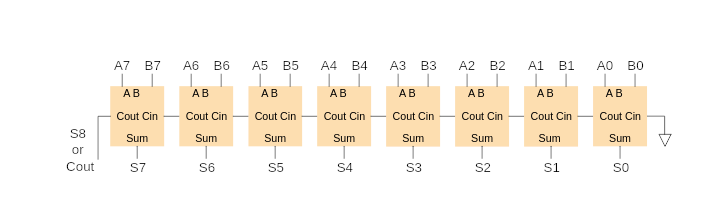
\includegraphics[width = 0.7\linewidth]{./image/ripple_carry_structure.png}
	\caption{Cấu trúc bộ Ripple Carry Adder}
	\label{f_diagam ripple carry adder}
\end{figure}

Trong đó:\\
\begin{itemize}[label = -]
	\item Tổng ($S_{i}$): $S_{i} = A_{i} \oplus B_{i} \oplus C_{i}$.
	\item Carry ($C_{i+1}$): $C_{i+1} = (A_{i} \& B_{i}) + (C_{i} \& (A_{i} \oplus B_{i}))$ 
\end{itemize}

\begin{itemize}[label = -]
	\item Ưu điểm: 
		\begin{itemize}[label = +]
			\item Thiết kế đơn giản, mỗi bit được xử lý bằng bộ Full Adder được kết nối theo chuỗi.
			\item Tiết kiệm tài nguyên phần cứng, phù hợp cho các hoạt động không yêu cầu quá cao về hiệu suất.
			\item Dễ dàng mở rộng mà không cần thay đổi quá nhiều vào logic của mạch.
			\item Tiết kiệm chi phí vì sử dụng ít cổng logic.
		\end{itemize}
	\item Nhược điểm:
		\begin{itemize}[label = +]
			\item Độ trễ cao do phải xử lý tuần tự, độ trễ tăng tuyến tính theo n-bit, với độ trễ được tính bằng \[ T_{delay} = n \times T_{unit} \] với, $T_{unit}$ là độ trễ của từng khối trong RCA.
			\item Hiệu suất thấp đối với số lượng bit lớn.
			\item Không tối ưu khi hệ thống yêu cầu thời gian thực vì có độ trễ lớn.
			\item Giới hạn hoạt động do tính tuần tự nên hệ thống RCA bị giới hạn tần số hoạt động, không đáp ứng ở hệ thống hoạt động ở tần số cao.
		\end{itemize}
\end{itemize}

\begin{lstlisting}[style = SystemVerilog, caption={RCA}]
	module rca (
	input logic [31:0]  i_data_a,  // Operand A
	input logic [31:0]  i_data_b,  // Operand B
	output logic [31:0] o_data     // Sum output
	);
	
	logic [31:0] carry; // Carry signals
	
	// Instance of the first full adder (LSB)
	full_adder FA0 (
	.i_data_a(i_data_a[0]),
	.i_data_b(i_data_b[0]),
	.i_carry(1'b0),          // Initial carry-in is 0
	.o_data(o_data[0]),
	.o_carry(carry[0])
	);
	
	// Instances of remaining 31 full adders
	full_adder FA1  (.i_data_a(i_data_a[1]),  .i_data_b(i_data_b[1]),  .i_carry(carry[0]), .o_data(o_data[1]),  .o_carry(carry[1]));
	full_adder FA2  (.i_data_a(i_data_a[2]),  .i_data_b(i_data_b[2]),  .i_carry(carry[1]), .o_data(o_data[2]),  .o_carry(carry[2]));
	full_adder FA3  (.i_data_a(i_data_a[3]),  .i_data_b(i_data_b[3]),  .i_carry(carry[2]), .o_data(o_data[3]),  .o_carry(carry[3]));
	full_adder FA4  (.i_data_a(i_data_a[4]),  .i_data_b(i_data_b[4]),  .i_carry(carry[3]), .o_data(o_data[4]),  .o_carry(carry[4]));
	full_adder FA5  (.i_data_a(i_data_a[5]),  .i_data_b(i_data_b[5]),  .i_carry(carry[4]), .o_data(o_data[5]),  .o_carry(carry[5]));
	full_adder FA6  (.i_data_a(i_data_a[6]),  .i_data_b(i_data_b[6]),  .i_carry(carry[5]), .o_data(o_data[6]),  .o_carry(carry[6]));
	full_adder FA7  (.i_data_a(i_data_a[7]),  .i_data_b(i_data_b[7]),  .i_carry(carry[6]), .o_data(o_data[7]),  .o_carry(carry[7]));
	full_adder FA8  (.i_data_a(i_data_a[8]),  .i_data_b(i_data_b[8]),  .i_carry(carry[7]), .o_data(o_data[8]),  .o_carry(carry[8]));
	full_adder FA9  (.i_data_a(i_data_a[9]),  .i_data_b(i_data_b[9]),  .i_carry(carry[8]), .o_data(o_data[9]),  .o_carry(carry[9]));
	full_adder FA10 (.i_data_a(i_data_a[10]), .i_data_b(i_data_b[10]), .i_carry(carry[9]), .o_data(o_data[10]), .o_carry(carry[10]));
	full_adder FA11 (.i_data_a(i_data_a[11]), .i_data_b(i_data_b[11]), .i_carry(carry[10]), .o_data(o_data[11]), .o_carry(carry[11]));
	full_adder FA12 (.i_data_a(i_data_a[12]), .i_data_b(i_data_b[12]), .i_carry(carry[11]), .o_data(o_data[12]), .o_carry(carry[12]));
	full_adder FA13 (.i_data_a(i_data_a[13]), .i_data_b(i_data_b[13]), .i_carry(carry[12]), .o_data(o_data[13]), .o_carry(carry[13]));
	full_adder FA14 (.i_data_a(i_data_a[14]), .i_data_b(i_data_b[14]), .i_carry(carry[13]), .o_data(o_data[14]), .o_carry(carry[14]));
	full_adder FA15 (.i_data_a(i_data_a[15]), .i_data_b(i_data_b[15]), .i_carry(carry[14]), .o_data(o_data[15]), .o_carry(carry[15]));
	full_adder FA16 (.i_data_a(i_data_a[16]), .i_data_b(i_data_b[16]), .i_carry(carry[15]), .o_data(o_data[16]), .o_carry(carry[16]));
	full_adder FA17 (.i_data_a(i_data_a[17]), .i_data_b(i_data_b[17]), .i_carry(carry[16]), .o_data(o_data[17]), .o_carry(carry[17]));
	full_adder FA18 (.i_data_a(i_data_a[18]), .i_data_b(i_data_b[18]), .i_carry(carry[17]), .o_data(o_data[18]), .o_carry(carry[18]));
	full_adder FA19 (.i_data_a(i_data_a[19]), .i_data_b(i_data_b[19]), .i_carry(carry[18]), .o_data(o_data[19]), .o_carry(carry[19]));
	full_adder FA20 (.i_data_a(i_data_a[20]), .i_data_b(i_data_b[20]), .i_carry(carry[19]), .o_data(o_data[20]), .o_carry(carry[20]));
	full_adder FA21 (.i_data_a(i_data_a[21]), .i_data_b(i_data_b[21]), .i_carry(carry[20]), .o_data(o_data[21]), .o_carry(carry[21]));
	full_adder FA22 (.i_data_a(i_data_a[22]), .i_data_b(i_data_b[22]), .i_carry(carry[21]), .o_data(o_data[22]), .o_carry(carry[22]));
	full_adder FA23 (.i_data_a(i_data_a[23]), .i_data_b(i_data_b[23]), .i_carry(carry[22]), .o_data(o_data[23]), .o_carry(carry[23]));
	full_adder FA24 (.i_data_a(i_data_a[24]), .i_data_b(i_data_b[24]), .i_carry(carry[23]), .o_data(o_data[24]), .o_carry(carry[24]));
	full_adder FA25 (.i_data_a(i_data_a[25]), .i_data_b(i_data_b[25]), .i_carry(carry[24]), .o_data(o_data[25]), .o_carry(carry[25]));
	full_adder FA26 (.i_data_a(i_data_a[26]), .i_data_b(i_data_b[26]), .i_carry(carry[25]), .o_data(o_data[26]), .o_carry(carry[26]));
	full_adder FA27 (.i_data_a(i_data_a[27]), .i_data_b(i_data_b[27]), .i_carry(carry[26]), .o_data(o_data[27]), .o_carry(carry[27]));
	full_adder FA28 (.i_data_a(i_data_a[28]), .i_data_b(i_data_b[28]), .i_carry(carry[27]), .o_data(o_data[28]), .o_carry(carry[28]));
	full_adder FA29 (.i_data_a(i_data_a[29]), .i_data_b(i_data_b[29]), .i_carry(carry[28]), .o_data(o_data[29]), .o_carry(carry[29]));
	full_adder FA30 (.i_data_a(i_data_a[30]), .i_data_b(i_data_b[30]), .i_carry(carry[29]), .o_data(o_data[30]), .o_carry(carry[30]));
	full_adder FA31 (.i_data_a(i_data_a[31]), .i_data_b(i_data_b[31]), .i_carry(carry[30]), .o_data(o_data[31]), .o_carry()); // Final carry ignored
	
	endmodule
	
	module full_adder(
	input logic     i_data_a,
	input logic     i_data_b,
	input logic     i_carry,
	
	output logic    o_data,
	output logic    o_carry
	);
	
	wire xor1;
	
	assign xor1 = i_data_a ^ i_data_b;
	assign o_data = xor1 ^ i_carry;
	assign o_carry = (i_data_a & i_data_b) | (i_carry & xor1);
	
	endmodule
\end{lstlisting}

\begin{lstlisting}[style = C, caption={Kết quả của test}]
	$ ./obj_dir/Vrca
	=== Test bench for Ripple Carry Adder (RCA) ===
	[PASS] Test case 1: A = 149, B = 186, Expected = 335, Actual = 335
	[PASS] Test case 2: A = 143, B = 254, Expected = 397, Actual = 397
	[PASS] Test case 3: A = 4, B = 0, Expected = 4, Actual = 4
	...
	[PASS] Test case 97: A = 165, B = 214, Expected = 379, Actual = 379
	[PASS] Test case 98: A = 120, B = 128, Expected = 248, Actual = 248
	[PASS] Test case 99: A = 116, B = 42, Expected = 158, Actual = 158
	[PASS] Test case 100: A = 36, B = 2, Expected = 38, Actual = 38
	
	=== Test Summary ===
	Total Test Cases: 100
	PASS: 100
	FAIL: 0
\end{lstlisting}
